%%%%%%%%%%%%%%%%%%%%%%%%%%%%%%%%%%%%%%%%%%%%%%%%%%%%%%%%%%%%%%%%%%%%%%%%%%%%%
% Chapter 7: Presupuesto
%%%%%%%%%%%%%%%%%%%%%%%%%%%%%%%%%%%%%%%%%%%%%%%%%%%%%%%%%%%%%%%%%%%%%%%%%%%%%%%

%++++++++++++++++++++++++++++++++++++++++++++++++++++++++++++++++++++++++++++++


La siguiente tabla de la Figura \ref{fig:presupuesto} nos indica cuantas horas de trabajo e investigación abarcó cada caracteristicas o funcionalidad de la aplicación, al igual que 
el número total de horas que duró el desarrollo de la aplicación GScout.

\begin{figure}[H]
\begin{center}
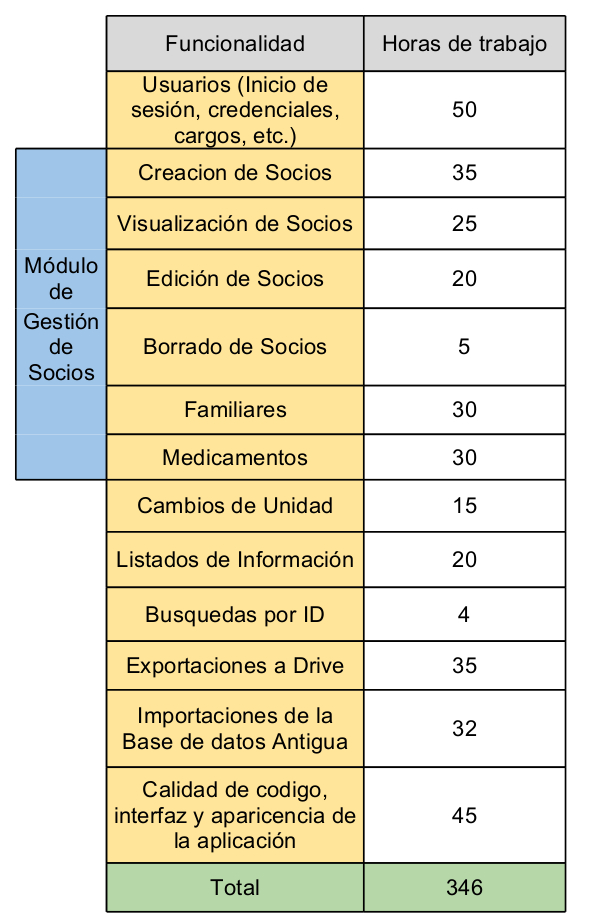
\includegraphics[width=0.47\textwidth]{images/presupuesto.jpg}
\caption{Números de horas totales y por funcionalidad que se llevaron a cabo en el proyecto}
\label{fig:presupuesto}
\end{center}
\end{figure}


